\chapter{HDMI}\label{chap:chap3}

Este capítulo descreve o trabalho realizado para cumprir a primeira parte do projeto: obter uma conexão HDMI entre recetor e transmissor. São descritas as várias configurações das placas HDMI disponiveis e ainda as arquiteturas desenvolvidas e implementadas para cumprir esta parte do projeto. 

\section{\textit{Hardware} utilizado}

Tal como mencionado no sub-capítulo \ref{sec:HDMIinFPGA}, para receber os dados provenientes do cabo HDMI e fazer a sua selecção são utilizadas duas placas HDMI (TB-FMCH-HDMI2 RX E TB-FMCH-HDMI2 TX) que, através das suas entradas e saída FMC de alta velocidade, conseguem enviar para a FPGA os sinais de imagem e som. Nas imagens \ref{fig:rx} e \ref{fig:tx} é possivel visualizar o recetor (TB-FMCH-HDMI2 RX) e o transmissor (TB-FMCH-HDMI2 TX) HDMI utilizados neste projeto. Em conjunto, estas duas placas são designadas apenas por TB-FMCH-HDMI2. Estas mesmas placas são constituidas por conectores HDMI, de seguida o sinal é enviado para um recetor ou transmissor HDMI, ADV7612 no caso do recetor e ADV7511 no caso do transmissor. Finalmente os sinais provenientes do recetor/transmissor são enviados para uma FGPA embebida na placa (XC6SLX45-3FGG484C) que, consoante a sua configuração, envia pelos conectores FMC os sinais de audio e video.

As placas possuem ainda uma PROM (\textit{Programmable read-only memory}) XCF16PFSG48C de configuração reprogramável que permite armazenar o \textit{bitstream} que configura a FPGA embebida do modo que se pretende. É esta FPGA embebida que em cada placa (RX e TX) é responsável pela selecção e envio dos dados pretendidos para os conectores FMC (e posterior envio para a FPGA), e como tal é necessário que estejam configuradas para realizarem tais procedimentos. O recurso a estas memórias reconfiguraveis vem permitir uma fácil alteração da configuração da FPGA uma vez que, segundo \cite{R026}, estas memórias de leitura permitem não só armazenar os \textit{bitstreams} de configuração da FPGA, mas também reconfigurá-los, caso se pretenda, de uma forma fácil e eficiente.

\subsection{Configurações da FPGA} \label{subsec:HDMIconfig}

A FPGA \textit{Spartan-6} (XC6SLX45-3FGG484C) embebida nas placas tem 3 configurações disponiveis. Estas configurações variam não só no suporte que têm, que pode ser apenasde imagem mas também de imagem e audio, mas variam também no número de bits por imagem que estas podem ter. Nas secções seguintes serão brevemente expostas as configurações disponiveis e como se pode tirar partido das mesmas no projeto.

--> Falar como é que se reconfigurou as placas
\subsubsection{Configuração por \textit{default}} \label{subsubsec:HDMIconfigdefault}

Esta configuração vem previamente escrita na memória PROM de fábrica e acaba por ser a mais simples de todas. Os dados enviados pelos conectores FMC são apenas referentes aos dados de imagem. As tabela \ref{table:HDMIdataRX} e \ref{table:HDMIdataTX} nas páginas \pageref{table:HDMIdataRX} e \pageref{table:HDMIdataTX} respectivamente identificam os pinos aos quais são atribuídas os sinais de dados de imagem HDMI tanto no recetor como no transmissor.

Esta configuração apenas transmite imagens RGB (\textit{Red Green Blue}) com 10 bits. Assim sendo, tal como referido em \cite{R009}, independentemente da formatação das imagens da fonte HDMI o recetor ADV7612 integrado na placa recetora HDMI converte a imagem para o formato RGB e transmite de maneira a enviar os dados em apenas 10 bits.  FALAR SOBRE ESTAS CONVERSÕES

A tabela \ref{table:HDMIdefaultSimplified} da página \pageref{table:HDMIdefaultSimplified}, adaptada de \cite{R009}, apresenta brevemente quais as portas das placas utilizadas e que sinais são transmitidos nas mesmas, no entanto é possivel encontrar na tabela \ref{table:HDMIdataDefaultdetail} do anexo \ref{ap1:HDMI} mais promenores relativamente a estes dados. Os nomes dos sinais são referentes aos sinais em TB-FMCH-HDMI2 (tanto TX como RX), assim como quando se faz referência à FPGA nestas tabelas estas correspondem às que estão embebidas nas placas HDMI. 

\begin{table}[h!]
	\centering
	\begin{tabular}{|c|c|c|c|}
		\hline
		\textbf{PIN}                                                                     & \textbf{FPGA -> FMC (RX)}                                                  & \textbf{FMC -> (TX)}                                                    & \textbf{Descrição}                                                      \\ \hline
		CLK0\_M2C\_P                                                                     & RX\#O\_LLC                                                                            & TX\#O\_DCLK                                                                           & \begin{tabular}[c]{@{}c@{}}Sinal de relógio dos\\   pixeis\end{tabular} \\ \hline
		LA00\_P\_CC                                                                      & RX\#0\_VSYNC                                                                          & TX\#0\_VSYNC                                                                          & \begin{tabular}[c]{@{}c@{}}Sincronização\\   Vertical\end{tabular}      \\ \hline
		LA01\_P\_CC                                                                      & RX\#0\_HSYNC                                                                          & TX\#0\_HSYNC                                                                          & \begin{tabular}[c]{@{}c@{}}Sincronização\\   Horizontal\end{tabular}    \\ \hline
		LA02\_P                                                                          & RX\#0\_DE                                                                             & TX\#0\_DE                                                                             & \begin{tabular}[c]{@{}c@{}}Sinal de \\ dados ativos\end{tabular}        \\ \hline
		\multirow{3}{*}{\begin{tabular}[c]{@{}c@{}}LA03\_P \\ a \\ LA32\_P\end{tabular}} & \multirow{3}{*}{\begin{tabular}[c]{@{}c@{}}RX\#0\_P0 \\ a \\ RX\#0\_P29\end{tabular}} & \multirow{3}{*}{\begin{tabular}[c]{@{}c@{}}TX\#0\_D0 \\ a \\ TX\#0\_D29\end{tabular}} & \multirow{3}{*}{Pixel de Imagem}                                        \\
		&                                                                                       &                                                                                       &                                                                         \\
		&                                                                                       &                                                                                       &                                                                         \\ \hline
	\end{tabular}
	\caption{Descrição e localização dos pinos de TB-FMCH-HDMI2 configurada por \textit{default}}
	\label{table:HDMIdefaultSimplified}
\end{table}

É de notar ainda que esta configuração é capaz de suportar até dois canais (RX0 e TX0, RX1 e TX1), no entanto nesta tabela apenas são apresentados os dados correspondentes ao canal 0 pois apenas será necessário utilizar um canal neste projeto. 

Apesar de ser um configuração simples, uma vez que apenas são transmitidos sinais de imagem em formato RGB, é uma configuração que será utilizada numa fase inicial em algumas arquiteturas implementadas que serão descritas no subcapitulo \ref{subsec:HDMIarquiteturas}.

\subsubsection{1 canal e suporte de audio} \label {subsubsec:HDMIconfig+audio}

Para além da configuração descrita anteriormente em \ref{subsubsec:HDMIconfigdefault} que apenas suporta a transmissão de imagem, existe ainda uma configuração capaz de suportar não só a transmissão de imagem mas também de som. A configuração que é escrita na PROM para programar a FPGA embebida controla o recetor ADV7612 de maneira a conseguir transmitir imagens no formato YCbCr ou RGB com 12 bits e também fazer a transmissão do audio em formato $I^{2}$S.

Assim como referido em \cite{R014}, neste caso a configuração da imagem está dependente da fonte HDMI, e é transmitida pelas placas tal como é emitida pela fonte, por outras palavras, se a fonte HDMI transmitir uma imagem em formato RGB é nesse formato que chega ao destino, no entanto se for transmitida uma imagem no formato YCbCr é nesse formato que chega ao seu destino. No caso do som, este é sempre transmitido em formato $I^{2}$S, o que implica a transmissão dos dados de audio mas também sinais de relógio necessários à sua transmissão. A tabela x passa a descrever com mais detalhe os sinais transmitidos para esta configuração da FPGA.

Na tabela \ref{table:HDMIaudiosuportSimplified} na página \pageref{table:HDMIaudiosuportSimplified} são brevemente apresentados as portas e os sinais usados com este tipo de configuração da FPGA embebida. Na tabela \ref{table:HDMI1canal+audioDETAIL} no anexo \ref{ap1:HDMI} é apresentada uma tabela semelhante a esta, mas que inclui mais detalhes relativamente aos pinos usados e ao seu uso. Ambas as tabelas foram adaptadas de \cite{R014} onde é são apresentados todos os detalhes dos conectores FMC das placas.

\begin{table}[h!]
	\centering
	\begin{tabular}{|c|c|c|c|}
		\hline
		\textbf{PIN}                                                                           & \textbf{FPGA -\textgreater FMC (RX)}                                                 & \textbf{FMC -> FPGA (TX)}                                                 & \textbf{FPGA->HDMI\_TX}                                                           \\ \hline
		CLK0\_M2C\_P                                                                           & RX\#0\_LLC                                                                           & TX\#0\_DCLK                                                                          & \begin{tabular}[c]{@{}c@{}}Sinal de relógio dos\\ pixeis\end{tabular}                        \\ \hline
		LA00\_P\_CC                                                                            & RX\#0\_VSYNC                                                                         & TX\#0\_VSYNC                                                                         & Sincronização vertical                                                                       \\ \hline
		LA01\_P\_CC                                                                            & RX\#0\_HSYNC                                                                         & TX\#0\_HSYNC                                                                         & Sincronização horizontal                                                                     \\ \hline
		LA02\_P                                                                                & RX\#0\_DE                                                                            & TX\#0\_DE                                                                            & Sinal de dados ativos                                                                        \\ \hline
		\multirow{3}{*}{\begin{tabular}[c]{@{}c@{}}LA03\_P\\   a LA32\_P\end{tabular}}         & \multirow{3}{*}{RX\#0\_P0 a RX\#0\_P29}                                              & \multirow{3}{*}{TX\#0\_D0 a TX\#0\_D29}                                              & \multirow{3}{*}{\begin{tabular}[c]{@{}c@{}}Pixel de imagem do bit\\   0 ao 29\end{tabular}}  \\
		&                                                                                      &                                                                                      &                                                                                              \\
		&                                                                                      &                                                                                      &                                                                                              \\ \hline
		\multirow{2}{*}{\begin{tabular}[c]{@{}c@{}}LA00\_N\_CC\\   a LA01\_N\_CC\end{tabular}} & \multirow{2}{*}{RX\#0\_InputVideoStatus}                                             & \multirow{2}{*}{TX\#0\_InputVideoStatus}                                             & \multirow{2}{*}{\begin{tabular}[c]{@{}c@{}}Formato de video\\   (2D/3D)\end{tabular}}        \\
		&                                                                                      &                                                                                      &                                                                                              \\ \hline
		LA19\_N                                                                                & RX\#0\_MCLK                                                                          & TX\#0\_MCLK                                                                          & \textit{Master Clock} de som                                                                          \\ \hline
		LA20\_N                                                                                & RX\#0\_SCLK                                                                          & TX\#0\_SCLK                                                                          & \textit{Serial Clock} de som                                                                          \\ \hline
		\multirow{2}{*}{\begin{tabular}[c]{@{}c@{}}LA21\_N\\   a LA26\_N\end{tabular}}         & \multirow{2}{*}{RX\#0\_AP0 a RX\#0\_AP5}                                             & \multirow{2}{*}{TX\#0\_AP0 a TX\#0\_AP5}                                             & \multirow{2}{*}{Dados de som}                                                                \\
		&                                                                                      &                                                                                      &                                                                                              \\ \hline
		\multirow{2}{*}{\begin{tabular}[c]{@{}c@{}}LA27\_N\\   a LA32\_N\end{tabular}}         & \multirow{2}{*}{\begin{tabular}[c]{@{}c@{}}RX\#0\_P30 a\\   RX\#0\_P35\end{tabular}} & \multirow{2}{*}{\begin{tabular}[c]{@{}c@{}}TX\#0\_P30 a\\   TX\#0\_P35\end{tabular}} & \multirow{2}{*}{\begin{tabular}[c]{@{}c@{}}Pixel de imagem do bit\\   30 ao 35\end{tabular}} \\
		&                                                                                      &                                                                                      &                                                                                              \\ \hline
	\end{tabular}
	\centering
	\caption{Descrição e localização dos pinos de TB-FMCH-HDMI2 configurada para 1 canal com suporte de audio}
	\label{table:HDMIaudiosuportSimplified}
\end{table}

Os dados referentes ao som transmitidos pela placa recetor HDMI e recebidos de seguida pela placa emissora HDMI estão mencionados com mais detalhe na tabela \ref{table:HDMI1canal+audioDETAIL}, e tal como indicado anteriormente, esta configuração é capaz de transmitir e receber dados no formato $I^{2}$S. Nas especificações deste protocolo, em \cite{R027}, são definidos os sinais transmitidos aquando a utilização deste formato, que passam a ser descritos:

\begin{enumerate}
	\item \textbf{\textit{Continuous Serial Clock} (SCK):} Este sinal é por vezes reconhecido pelo nome de \textit{Bit Clock} e é um sinal de relógio referente aos dados de som em série transmitidos pelos canais AP1, AP2, AP3 e AP4.
	
	\item \textbf{\textit{Word Select}(WS)}: Este sinal é por vezes também conhecido por \textit{Left/Right Clock} e é um sinal que indica o canal de som (esquerdo ou direito) que está a ser transmitido através dos dados em série recebidos ou enviados nas portas AP1, AP2, AP3 e AP4. É nomeado de sinal de relógio porque geralmente alterna entre 0 e 1 periodicamente, no entanto tal pode não acontecer, tal como referido em \cite{R027}. 
	
	\item \textbf{\textit{Serial Data}}: Sinais que transportam os dados de audio.

\end{enumerate}

Na imagem \ref{fig:i2s_audio} são ilustrados os sinais referentes ao audio descritos previamente. O sinal "SCLK" (\textit{Serial Clock}) é referente ao sinal "\textit{Continuous Serial Clock}", o sinal LRCLK (\textit{Left/Right Clock}) refere-se ao sinal "\textit{Word Select}" e ainda ISx refere-se ao sinal "\textit{Serial Data}".
	\begin{figure}[h!]
	\begin{center}
		\leavevmode
		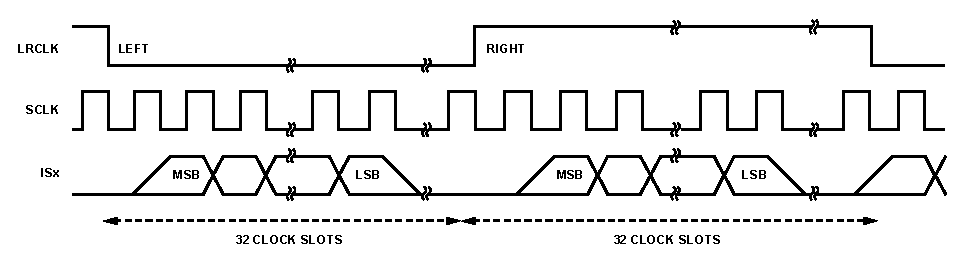
\includegraphics[width=1.0\textwidth]{audio_i2s}
		\caption{Ilustração dos sinais de som transmitidos no formato $I^{2}$S, retirada de \cite{R016}}
		\label{fig:i2s_audio}
	\end{center}
\end{figure}

Na placa recetora HDMI, que envia os dados para a FPGA Virtex-7, é também enviado o sinal \textit{Master Clock} que corresponde a um sinal de relógio de referência do sinais de audio da entrada e ainda dados de audio em AP0. É mencionado em \cite{R016} que estes dois sinais são referentes ao formato SPDIF e como tal não serão abordados neste projeto uma vez que as placas apenas suportam o formato $I^{2}$S.

Esta configuração das FPGAs embebidas nas placas é a configuração mais utilizada ao longo do projeto, uma vez que para além de ser versátil quanto ao formato das imagens transmitidas, é também capaz de suportar audio. Em contrapartida, apenas suporta um canal (ao contrário da anterior), mas tal não é um problema pois apenas se pretende obter uma transmissão num único canal entre dispositivo de fonte HDMI e dispositivo final HDMI. 


\subsubsection{2 canais melhorado} \label{subsubsec:HDMIconfigMelhorado}

--> Dizer que esta configuração faz tal tal e tal, mas que não será abordad uma vez que nao foi utilizada

\subsection{Configuração dos \textit{switches}}

Explicar como configurar os switches para obter o que queremos

\subsection{Arquiteturas Desenvolvidas} \label{subsec:HDMIarquiteturas}

Neste sub-capitulo passam a ser descritos as arquiteturas desenvolvidas e implementadas na FPGA apenas referente à comunicação entre as placas HDMI. 

\subsubsection{Transmissão de uma imagem gerada na FPGA}

Inicialmente optou-se pela geração de uma imagem na FPGA e o seu envio para a placa transmissora HDMI através dos conectores FMC.

		\begin{figure}[h!]
	\begin{center}
		\leavevmode
		\includegraphics[width=1.0\textwidth]{planA}
		\caption{}
		\label{fig:planA}
	\end{center}
\end{figure}

\subsubsection{Transmissão de imagem entre dispositivos HDMI}

		\begin{figure}[h!]
	\begin{center}
		\leavevmode
		\includegraphics[width=1.0\textwidth]{planB1}
		\caption{}
		\label{fig:planb1}
	\end{center}
\end{figure}

\subsubsection{Transmissão de imagem e som entre dispositivos HDMI}